% Setting up the document class for IEEE conference format
\documentclass[conference]{IEEEtran}
\IEEEoverridecommandlockouts

% Including essential packages for document formatting and content
\usepackage{amsmath,amsfonts}
\usepackage{graphicx}
\usepackage{booktabs}
\usepackage{hyperref}
\usepackage{cite}
\usepackage{algorithm}
\usepackage{algpseudocode}
\usepackage{xcolor}

% Configuring bibliography style
\bibliographystyle{IEEEtran}

% Setting up fonts (using standard LaTeX fonts to ensure compatibility)
%\usepackage{times}

\begin{document}

% Defining the title and authors with team details
\title{Advanced Machine Learning for Business Transformation: Project Instructions \& Template}
\author{
    \IEEEauthorblockN{John Smith, Jane Doe, Alex Johnson}
    \IEEEauthorblockA{Goa Institute of Management\\
    Big Data Analytics\\
    Student IDs: \{123456, 789012, 345678\}\\
    Email: \{john.smith, jane.doe, alex.johnson\}@gim.ac.in}
}

\date{\today}

% Creating the title
\maketitle

% Abstract section
\begin{abstract}
This paper presents a machine learning project addressing a specific business problem. The study outlines the problem's relevance, significance, and originality, followed by a detailed methodology, results, and analysis. Adhering to IEEE format, the project ensures clarity, reproducibility, and technical rigor. Key findings demonstrate the proposed solution's impact on the business domain, supported by appropriate evaluation metrics and visualizations.
\end{abstract}

% Keywords section
\begin{IEEEkeywords}
Machine Learning, Business Applications, Data Analysis, Predictive Modeling, IEEE Format
\end{IEEEkeywords}

% Introduction section
\section{Introduction}
% Establishing the business problem and its context
The business problem addressed in this paper is Your Business Problem. This section introduces the problem's context, its relevance to the business domain, and the motivation for applying machine learning techniques. The significance of solving this problem is justified by its potential impact on Your Business Impact, such as improved efficiency or enhanced decision-making.

% Defining the scope and objectives
\subsection{Scope and Objectives}\label{subsub:lists}
The project aims to Your Project Goal. The objectives include:
\begin{itemize}
    \item Establishing the relevance of the problem to the business domain.
    \item Demonstrating originality in the problem formulation or methodology.
    \item Achieving robust results through sound machine learning techniques.
    \item Ensuring reproducibility and transparency in data and methods.
\end{itemize}

% Submission Requirements section
\section{Submission Requirements}
% Outlining the submission guidelines and deadlines
This project adheres to the following submission requirements and deadlines:
\begin{itemize}
    \item \textbf{Project Report}: The report is formatted in IEEE conference style, with a maximum length of 6 pages, including references, using the Overleaf IEEE Template.
    \item \textbf{Using the Overleaf Template}: To start your project, follow these steps:
    \begin{itemize}
        \item Access the template at \url{https://www.overleaf.com/read/vqqhmbkrrkqj#3a07de}, which opens in read-only mode.
        \item Click ``Menu" (top left, above the file list).
        \item Select "Copy Project" from the dropdown to create a private version for your group.
        \item Rename the project (e.g., Group3\_SalesForecasting) and begin editing.
        \item Do not edit the original read-only template, as it is shared by all groups. Ensure you work in your own copy.
    \end{itemize}
    \item \textbf{Team Details}: The team consists of John Smith (ID: 123456), Jane Doe (ID: 789012), and Alex Johnson (ID: 345678), with contact emails provided in the author block.
    \item \textbf{Code and Data}: The final code and cleaned dataset are uploaded to a GitHub repository, with links provided in Section~\ref{sec:reproducibility}.
    \item \textbf{Reproducibility Note}: A brief description of how to replicate core results is included in Section~\ref{sec:reproducibility}.
    \item \textbf{AI Use Declaration}: The use of AI tools is explicitly declared in Section~\ref{subsec:ai_use}, with AI-generated content (text or code) not exceeding 20\% as per Turnitin guidelines.
    \item \textbf{Submission Deadlines}:
    \begin{itemize}
        \item First Review Submission: 9th October, 2026
        \item Second Review Submission: 20th November, 2026
        \item Final Submission: 4th December, 2026
        \item All deadlines are 11:59 PM AoE
    \end{itemize}
\end{itemize}

% Related Work section
\section{Related Work}
\label{sec:related_work}
% Reviewing prior work and positioning the project
This section reviews existing literature and prior work related to Your Business Problem. Previous studies, such as Your Cited Work, have addressed similar problems but differ in Your Differentiation. The proposed approach builds on these works by incorporating Your Novel Contribution, ensuring originality and relevance to the business context.

% Methodology section
\section{Methodology}
% Describing the approach, data, and models
This section details the machine learning methodology, including data sources, preprocessing steps, model selection, and evaluation metrics, designed to ensure reproducibility and technical rigor.

% Subsection for data
\subsection{Data}
The dataset used is Your Dataset Description, sourced from Your Data Source. Preprocessing steps include Your Preprocessing Steps. The data is accessible at Your Data Repository Link, ensuring transparency.

% Subsection for models
\subsection{Models and Techniques}
The machine learning models employed include Your Models. The rationale for model selection is Your Model Selection Reasoning. Hyperparameters and training procedures are detailed to support reproducibility.

% Subsection for evaluation
\subsection{Evaluation Metrics}
The evaluation metrics used are Your Metrics, chosen because Your Metric Justification. These metrics align with the business objectives and provide a robust assessment of model performance.

% Results section
\section{Results}
% Presenting the results
The project achieved Your Key Results. Results are presented using tables and visualizations, as shown in Table~\ref{tab:example_table} and Figure~\ref{fig:results}.

% Example figure
\begin{figure}[h]
    \centering
    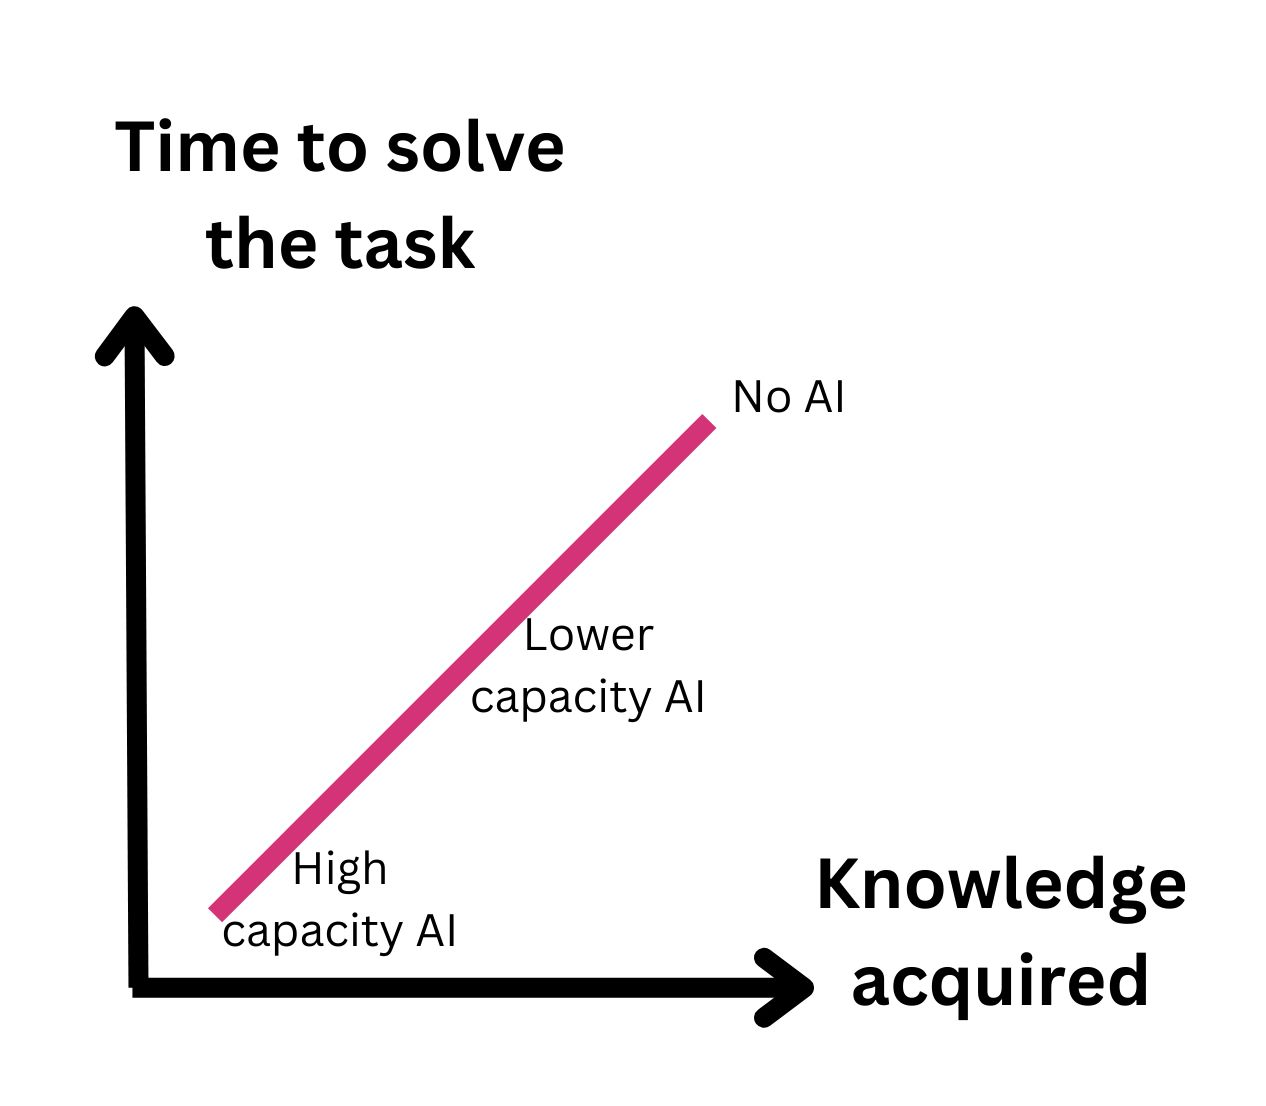
\includegraphics[width=0.9\columnwidth]{your_figure.png}
    \caption{Visualization of Model Performance}
    \label{fig:results}
\end{figure}

% Discussion section
\section{Discussion}
% Analyzing and interpreting results
The results indicate Your Result Analysis. The findings are compared to Your Baseline or Prior Work, highlighting the project's success in meeting its objectives. The business relevance is evident through Your Relevance Reasoning, and the significance is underscored by Your Impact Analysis. Originality is demonstrated by Your Novel Contribution, while technical quality is supported by Your Technical Justification. Limitations, such as Your Limitations, are acknowledged to provide a balanced perspective.

% Evaluation Rubric section
\section{Evaluation Rubric}
% Explaining the evaluation criteria
The project is evaluated based on the following rubric, which outlines the criteria, descriptions, and respective weights used to assess the work. The rubric ensures a comprehensive evaluation of the project's relevance, significance, originality, achievement, writing, reproducibility, and technical quality. The table spans both columns of the IEEE format and is centered for clarity. Refer Table~\ref{tab:rubric}.

\begin{table*}[t]
    \centering
    \caption{Evaluation Rubric for AMLBT Project}
    \label{tab:rubric}
    \begin{tabular}{p{3cm} p{12cm} c}
        \toprule
        \textbf{Criterion} & \textbf{Description} & \textbf{Weight} \\
        \midrule
        Relevance  & How clearly is the business relevance established? Is the problem context meaningful and well-justified? & 4 \\
        Significance  & How important is the problem to the business domain? Is there a valuable insight or impact if solved? & 4 \\
        Originality  & Does the project show creativity or novelty in either the problem selected or the ML approach used? & 6 \\
        Achievement  & How well did the team execute their plan? Are the results clearly presented, analyzed, and supported? & 4 \\
        Writing  & Is the report well-structured, clear, and professionally written in IEEE format? Are visuals and tables used effectively? & 4 \\
        Reproducibility & Are data, methodology, and code made transparent and accessible? Can someone else repeat the key steps? & 4 \\
        Technical Quality & Are the methods and models used sound? Are the evaluation metrics appropriate and correctly interpreted? & 4 \\
        \midrule
        \textbf{Total} & & \textbf{30} \\
        \bottomrule
    \end{tabular}
\end{table*}

% Prompts to Enhance AMLBT Project or Paper section
\section{Prompts to Enhance AMLBT Project or Paper}
% Providing prompts aligned with the evaluation rubric
To enhance the quality and alignment of the Advanced Machine Learning for Business Transformation (AMLBT) project and paper with the evaluation rubric, the following prompts are provided. These prompts are organized by the rubric criteria to guide the team in addressing each criterion effectively, ensuring a robust and high-quality submission.

\begin{itemize}
    \item \textbf{Relevance}
    \begin{itemize}
        \item How can we clearly articulate the business problem to demonstrate its alignment with the goals of Your Business Domain?
        \item What specific business metrics or outcomes will be improved by solving Your Business Problem using machine learning?
        \item How do we justify the problem's relevance to stakeholders in Your Industry with concrete examples or case studies?
    \end{itemize}
    \item \textbf{Significance}
    \begin{itemize}
        \item What are the potential long-term impacts of solving Your Business Problem on Your Business Domain?
        \item How can we quantify the value of insights gained from the machine learning solution for Your Business Context?
        \item What evidence from industry trends or prior work supports the importance of addressing Your Business Problem?
    \end{itemize}
    \item \textbf{Originality}
    \begin{itemize}
        \item How can we introduce a novel perspective or approach to Your Business Problem that differentiates it from existing solutions?
        \item What unique machine learning techniques or data combinations can we apply to enhance the creativity of our project?
        \item How do we demonstrate that our problem formulation or methodology offers new insights in Your Business Domain?
    \end{itemize}
    \item \textbf{Achievement}
    \begin{itemize}
        \item How can we clearly present our results to highlight the successful execution of our project plan?
        \item What visualizations or tables can best showcase the performance of our machine learning model for Your Business Problem?
        \item How do we analyze our results to provide actionable business insights for Your Business Context?
    \end{itemize}
    \item \textbf{Writing}
    \begin{itemize}
        \item How can we structure our paper to ensure clarity and adherence to IEEE conference format guidelines?
        \item What strategies can we use to make our writing more professional and concise for an academic audience?
        \item How do we effectively integrate visuals and tables to support our narrative and enhance readability?
    \end{itemize}
    \item \textbf{Reproducibility}
    \begin{itemize}
        \item What steps should we document to ensure another researcher can replicate our machine learning pipeline for Your Business Problem?
        \item How do we organize our GitHub repository to make data, code, and methodology transparent and accessible?
        \item What specific software versions or dependencies should we include to facilitate replication of our results?
        \item Include the GitHub repository link in the paper. 
    \end{itemize}
    \item \textbf{Technical Quality}
    \begin{itemize}
        \item How do we justify the appropriateness of our chosen machine learning models for Your Business Problem?
        \item What evaluation metrics are most suitable for assessing our model’s performance in Your Business Context, and why?
        \item How can we address potential limitations or biases in our methodology to strengthen technical rigor?
    \end{itemize}
    \item \textbf{Responsible Use of Prompts}
    \begin{itemize}
        \item Use these prompts to refine ideas and improve alignment with the rubric, not to generate the entire paper or code.
        \item Always review and edit AI-generated content for accuracy, relevance, and alignment with project goals.
        \item Include a note in the AI Use Declaration (Section~\ref{subsec:ai_use}) about any AI assistance used.
    \end{itemize}
\end{itemize}

% Literature Review and Bibliography Guidelines section
\section{Literature Review and Bibliography Guidelines}
% Providing guidance on conducting a literature review and managing bibliography
This section outlines the steps for conducting a literature review and creating a bibliography in IEEE format to ensure a robust Related Work section (Section~\ref{sec:related_work}) that supports the project's relevance, significance, and originality.

\subsection{Conducting a Literature Review}
To perform an effective literature review for Your Business Problem:
\begin{itemize}
    \item \textbf{Identify Relevant Sources}: Search academic databases (e.g., IEEE Xplore, Google Scholar, Scopus) using keywords related to Your Business Problem and machine learning. Focus on peer-reviewed papers, industry reports, and recent studies (within the last 5–10 years) in Your Business Domain.
    \item \textbf{Evaluate Source Quality}: Prioritize high-impact journals, conference proceedings, and reputable sources. Assess relevance to Your Business Problem and the credibility of the authors or institutions.
    \item \textbf{Synthesize Findings}: Summarize key findings, methodologies, and gaps in prior work. Group sources by themes (e.g., similar problems, machine learning techniques, or business applications) to provide a structured narrative.
    \item \textbf{Position Your Work}: Highlight how Your Novel Contribution addresses gaps or limitations in the literature, emphasizing the originality and significance of your project.
    \item \textbf{Cite Appropriately}: Use IEEE citation style for in-text citations and ensure all referenced works appear in the bibliography.
\end{itemize}

\subsection{Creating an IEEE-Format Bibliography}
The bibliography must follow IEEE format, as implemented in this template using the \texttt{thebibliography} environment and \texttt{bibliographystyle\{IEEEtran\}}. Guidelines include:
\begin{itemize}
    \item \textbf{Format Entries Correctly}: Each entry should include author(s), title, journal/conference name, volume, issue, pages, and year, formatted as shown in the References.
    \item \textbf{Order Citations Numerically}: Citations are numbered in the order they appear in the text (e.g., [1], [2]). Use \texttt{\textbackslash cite\{label\}} for in-text citations.
    \item \textbf{Use Reliable Sources}: Include only peer-reviewed or reputable sources relevant to Your Business Problem. Avoid non-scholarly or unverified references.
    \item \textbf{Manage References Efficiently}: Use a reference management tool (e.g., Zotero, Mendeley, Google Scholar) to organize sources and generate IEEE-compliant BibTeX entries, which can be adapted for the \texttt{thebibliography} environment.
    \item \textbf{Keep Within Page Limit}: Ensure the bibliography fits within the 4-page limit, prioritizing the most relevant references (typically 5–15 entries for a conference paper).
\end{itemize}

% Basic LaTeX Formatting Examples section
\section{Basic \LaTeX\ Formatting Examples}
% Providing examples of common LaTeX elements
This section provides examples of basic LaTeX formatting elements commonly used in IEEE conference papers, such as tables, mathematical equations, lists, and figures, to assist in presenting the AMLBT project effectively. For more documentation, refer to \url{https://www.overleaf.com/learn}.

\subsection{Table Example}
A simple table can be used to present data or results clearly. Below is an example of a table comparing model performance metrics.

\begin{table}[ht]
    \centering
    \caption{Example Model Performance Comparison}
    \label{tab:example_table}
    \begin{tabular}{l c c}
        \toprule
        Model & Accuracy (\%) & F1-Score \\
        \midrule
        Logistic Regression & 85.2 & 0.78 \\
        Random Forest & 88.7 & 0.82 \\
        \bottomrule
    \end{tabular}
\end{table}

\subsection{Math Equation Example}
Mathematical equations are often used to describe machine learning models or metrics. Below is an example of a logistic regression equation in LaTeX, formatted using the \texttt{amsmath} package.

\begin{equation}
    P(y=1|\mathbf{x}) = \frac{1}{1 + e^{-\mathbf{w}^T \mathbf{x} - b}}
    \label{eq:logistic}
\end{equation}

This equation represents the probability of a positive class in a logistic regression model, where \(\mathbf{x}\) is the feature vector, \(\mathbf{w}\) is the weight vector, and \(b\) is the bias term.

\subsection{List Example}
Lists are useful for summarizing steps, objectives, or findings. Below is an example of a bulleted list in IEEE format.

\begin{itemize}
    \item Preprocess the dataset by handling missing values and normalizing features.
    \item Train the model using a 70-30 train-test split.
    \item Evaluate the model using accuracy, precision, and recall metrics.
\end{itemize}

\subsection{Figure Placeholder Example}
Figures are essential for visualizing results. Below is an example of a figure placeholder, which can be adapted to include your project’s visualizations.

\begin{figure}[ht]
    \centering
    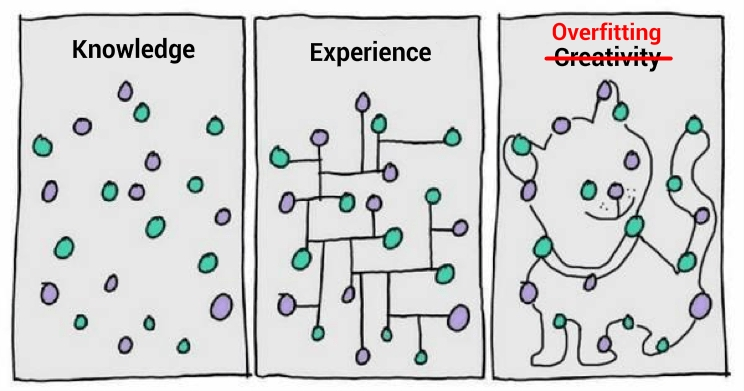
\includegraphics[width=0.9\columnwidth]{example_plot.png}
    \caption{Example Visualization of Model Predictions}
    \label{fig:example_figure}
\end{figure}

These examples demonstrate how to format common elements in LaTeX while adhering to IEEE guidelines. Adapt these structures to present Your Business Problem’s data, models, or results effectively.

% Reproducibility section
\section{Reproducibility}
\label{sec:reproducibility}
% Ensuring transparency and accessibility
The project ensures reproducibility by providing access to the data, code, and methodology. The code and cleaned dataset are available at Your GitHub Repository Link. To replicate the core results, follow the Reproducibility Steps (e.g., clone the repository, install dependencies listed in README.md, and run the main script). All dependencies and software versions are documented in the repository to facilitate replication.

% AI Use Declaration subsection
\subsection{AI Use Declaration}
\label{subsec:ai_use}
% Declaring AI tool usage
AI tools, such as Your AI Tool (e.g., ChatGPT, Copilot, Grok, etc.), were used for Your AI Usage Description (e.g., generating initial code drafts or refining text). Ensure AI-generated content (text or code) constitutes less than 20\% of the submission, as verified by Turnitin (\url{https://www.turnitin.com}), ensuring compliance with project guidelines.

% Conclusion section
\section{Conclusion}
% Summarizing the project and its impact
This project successfully addressed Your Business Problem using machine learning techniques. The results demonstrate Your Key Findings, with significant implications for Your Business Domain. Future work could explore Your Future Work Suggestions to further enhance the solution.

% Acknowledgment section
\section{Acknowledgment (Optional)}
% Thanking contributors and resources
The authors would like to thank Your Advisor or Instructor for their guidance and feedback throughout the project. We also acknowledge Your Institution for providing access to computational resources and Your Funding Source (if applicable) for financial support. Additionally, we appreciate the contributions of Your Collaborators or Peers who provided valuable insights during the development of this work.

% References section
\begin{thebibliography}{9}
\bibitem{journal_example}
A. B. Author and C. D. Author, ``Predicting Customer Churn Using Machine Learning Techniques,'' \emph{IEEE Transactions on Knowledge and Data Engineering}, vol. 35, no. 4, pp. 1234--1245, Apr. 2023.

\bibitem{conference_example}
E. F. Researcher, G. H. Analyst, and I. J. Developer, ``Demand Forecasting with Neural Networks for Retail Applications,'' in \emph{Proc. IEEE Int. Conf. Data Mining (ICDM)}, Beijing, China, Nov. 2024, pp. 567--572.

\bibitem{book_example}
K. L. Smith, \emph{Machine Learning for Business Analytics}, 2nd ed. New York, NY, USA: Wiley, 2022.

\bibitem{online_example}
M. N. Data, ``UCI Machine Learning Repository: Adult Income Dataset,'' \emph{UCI Machine Learning Repository}, 2023. [Online]. Available: \url{https://archive.ics.uci.edu/ml/datasets/adult}
\end{thebibliography}

\end{document}